
%-------------------------------------------------------------------------
\section{Results}
\label{section results}

We implement an integrated system using OpenCL 1.0 and QT 4.8.
Our system supports across heterogeneous platforms.
The experimental environment is: Windows 8 64bit with Intel (R) Core i7-3770 @ 3.40GHz and NVIDIA GeForce GTX TITAN @ 6GB (or AMD Radeon HD 7990 @ 2$\times$3GB).
Different kinds of data sets are used to evaluate our method, and we compare our algorithm with both CPU based methods and GPU based methods.

%-------------------------------------------------------------------------
\subsection{Datasets}

We tested two kinds of data sets.
One of them is a part of the benchmark provided by Grid-Cut \cite{12JSH}.
The other is downloaded from the Internet, which includes high-resolution images, HD videos and volume data sets.
Below is the detail information of the data sets and the scaled-up versions of the data sets.
The performance of different algorithms is summarized in \tablename \ \ref{table benchmark}.

\begin{table}
\center
\caption{Benchmark Datasets}
\label{table benchmark}
{
    \fontsize{6.5pt}{8pt}\selectfont
    \begin{tabular}{@{ }c|r|r@{ }r@{ }r|r|c@{ }}
    \hline\rule{0pt}{0.3cm}
    Name & Scale & Width & Height & Depth & Max Flow & Size (MB)\\
    \hline\rule{0pt}{0.30cm}
       \multirow{3}{*}{\specialcell{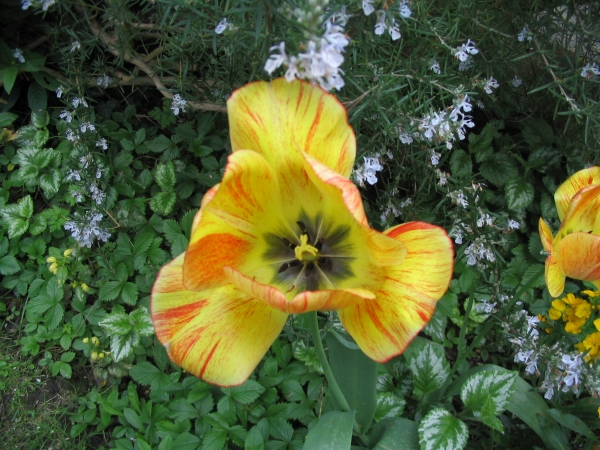
\includegraphics[width=0.70cm]{figures/fig5a.png}\\Flower(M)}}
       & 1 x 1     & 600   & 450   & 1     & 1208089    & 3.35\\
       & 4 x 4     & 2400  & 1800  & 1     & 7856011    & 53.5\\
       & 16 x 16   & 9600  & 7200  & 1     & 50618597   & 856 \\
    \hline\rule{0pt}{0.30cm}
       \multirow{3}{*}{\specialcell{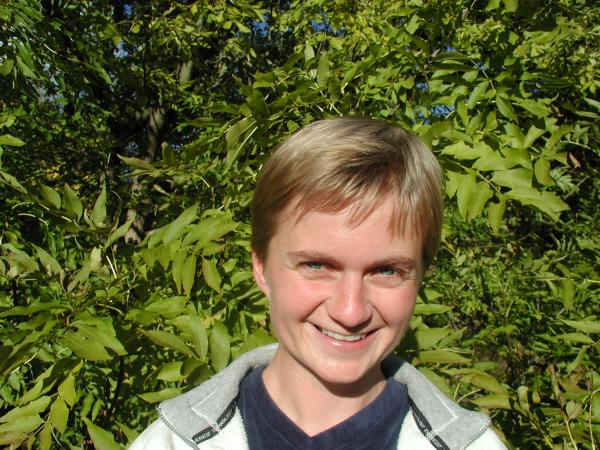
\includegraphics[width=0.70cm]{figures/fig5b.png}\\Person(M)}}
       & 1 x 1     & 600   & 450   & 1     & 880461     & 3.35\\
       & 4 x 4     & 2400  & 1800  & 1     & 5042635    & 53.5\\
       & 16 x 16   & 9600  & 7200  & 1     & 29042350   & 856 \\
    \hline\rule{0pt}{0.30cm}
       \multirow{3}{*}{\specialcell{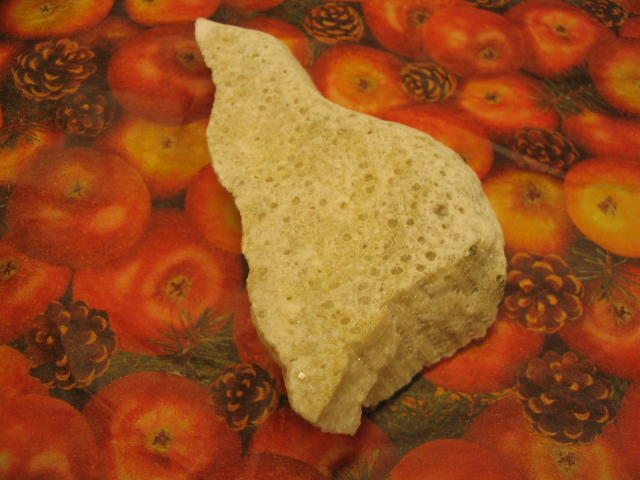
\includegraphics[width=0.70cm]{figures/fig5c.png}\\Sponge(M)}}
       & 1 x 1     & 640   & 480   & 1     & 343591     & 3.81\\
       & 4 x 4     & 2560  & 1920  & 1     & 1910718    & 60.9\\
       & 16 x 16   & 10240 & 7680  & 1     & 10136071   & 975 \\
    \hline\rule{0pt}{0.30cm}
       \multirow{3}{*}{\specialcell{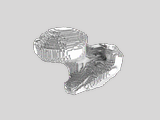
\includegraphics[width=0.70cm]{figures/fig5d.png}\\Bone(U)}}
       & 1 x 1 x 1 & 256   & 256   & 119   & 71344      & 111 \\
       & 2 x 2 x 2 & 512   & 512   & 238   & 1913780    & 892 \\
       &           &       &       &       &            &     \\
    \hline\rule{0pt}{0.30cm}
       \multirow{3}{*}{\specialcell{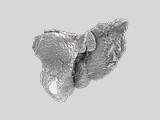
\includegraphics[width=0.70cm]{figures/fig5e.png}\\Liver(U)}}
       & 1 x 1 x 1 & 170   & 170   & 144   & 625447     & 59.5\\
       & 2 x 2 x 2 & 340   & 340   & 288   & 3886049    & 476 \\
       &           &       &       &       &            &     \\
    \hline\rule{0pt}{0.30cm}
       \multirow{3}{*}{\specialcell{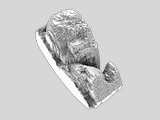
\includegraphics[width=0.70cm]{figures/fig5f.png}\\Babyface(U)}}
       & 1 x 1 x 1 & 250   & 250   & 81    & 222943     & 72.4\\
       & 2 x 2 x 2 & 500   & 500   & 162   & 3316927    & 579 \\
       &           &       &       &       &            &     \\
    \hline\rule{0pt}{0.30cm}
       \multirow{3}{*}{\specialcell{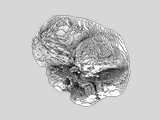
\includegraphics[width=0.70cm]{figures/fig5g.png}\\Adhead(U)}}
       & 1 x 1 x 1 & 256   & 256   & 192   & 589368     & 180 \\
       & 2 x 2 x 2 & 512   & 512   & 384   & 3594110    & 1440\\
       &           &       &       &       &            &     \\
    \hline\rule{0pt}{0.30cm}
       \multirow{3}{*}{\specialcell{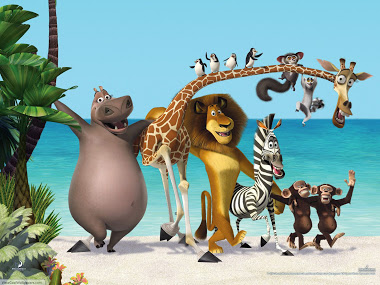
\includegraphics[width=0.70cm]{figures/fig5h.jpg}\\Madagascar(G)}}
       &           &       &       &       &            &      \\
       & 1 x 1 x 1 & 10800 & 8100  & 1     & 4946409834 & 1413 \\
       &           &       &       &       &            &      \\
    \hline\rule{0pt}{0.30cm}
       \multirow{3}{*}{\specialcell{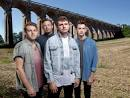
\includegraphics[width=0.70cm]{figures/fig5i.jpg}\\LTA(G)}}
       &           &       &       &       &            &      \\
       & 1 x 1 x 1 & 9900  & 7500  & 1     & 6244836523 & 1198 \\
       &           &       &       &       &            &      \\
    \hline\rule{0pt}{0.30cm}
       \multirow{2}{*}{\specialcell{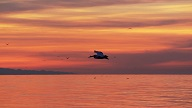
\includegraphics[width=0.70cm]{figures/fig5j.jpg}\\TimeScapes(Y)}}
       &           &       &       &       &            &      \\
       & 1 x 1 x 1 & 2560  & 1440  & 30    & 80886496   & 1577 \\
       &           &       &       &       &            &      \\
    \hline\rule{0pt}{0.30cm}
       \multirow{2}{*}{\specialcell{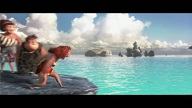
\includegraphics[width=0.70cm]{figures/fig5k.jpg}\\The Croods(Y)}}
       &           &       &       &       &            &      \\
       & 1 x 1 x 1 & 1920  & 1080  & 40    & 180301245  & 1178 \\
       &           &       &       &       &            &      \\
    \hline\rule{0pt}{0.30cm}
       \multirow{2}{*}{\specialcell{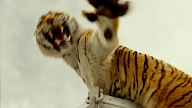
\includegraphics[width=0.70cm]{figures/fig5l.jpg}\\Life of PI(Y)}}
       &           &       &       &       &            &      \\
       & 1 x 1 x 1 & 1920  & 1080  & 32    & 1178329527 & 949  \\
       &           &       &       &       &            &      \\
    \hline\rule{0pt}{0.30cm}
       \multirow{3}{*}{\specialcell{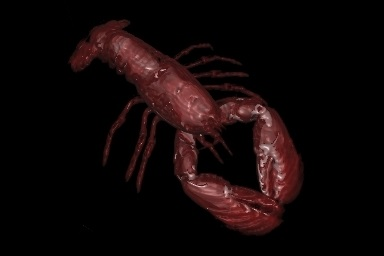
\includegraphics[width=0.70cm]{figures/fig5m.jpg}\\MRBrain(V)}}
       &           &       &       &       &            &      \\
       & 1 x 1 x 1 & 256   & 256   & 109   & 29036      & 102  \\
       &           &       &       &       &            &      \\
    \hline\rule{0pt}{0.30cm}
       \multirow{3}{*}{\specialcell{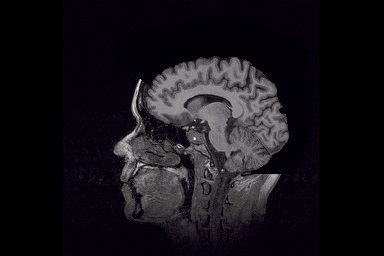
\includegraphics[width=0.70cm]{figures/fig5n.jpg}\\Lobster(V)}}
       &           &       &       &       &            &      \\
       & 1 x 1 x 1 & 301   & 324   & 56    & 238402     & 78   \\
       &           &       &       &       &            &      \\
    \hline\rule{0pt}{0.30cm}
    \end{tabular}
    \begin{tablenotes}
        \item {
        \begin{enumerate}
            \item M - Middlebury College: \url{http://vision.middlebury.edu/MRF/}
            \item U - University of Western Ontario: \url{http://vision.csd.uwo.ca/data/maxflow/}
            \item G - Google Advanced Image Search: \url{http://images.google.com/advanced_image_search}
            \item Y - YouTube: \url{http://www.youtube.com/}
            \item V - VolVis: \url{http://www.volvis.org/}
        \end{enumerate}}
    \end{tablenotes}
}
\end{table}

We conduct experiments on these large data sets to show the practicality and efficiency of our method.
In these experiments, the foreground and background are colored in magenta and green respectively, and the cut results are highlighted in yellow.

\paragraph*{\textbf{Image Segmentation}} The results include two parts, as shown in \figurename \ref{figure image segmentation}.
The first part contains standard data sets (from Middlebury) with providing energy function.
The
\textit{Lower Than Atlantis}
\footnotemark[1]\footnotetext[1]{\scriptsize Lower Than Atlantis: \url{http://fashionsoundtrack.com/wp-content/uploads/2013/08/A1posterLTA.jpg}} and
\textit{Madagascar}
\footnotemark[2]\footnotetext[2]{\scriptsize Madagascar: \url{http://wallpaper.imgcandy.com/images/233316-jessica-alba-wardrobe-malfunction-original-source-of-image.jpg}}
data sets in the second part are much larger and we use the clustering based model to set up energy function.

\begin{figure*}
\centering
\subfigure[Flower - $600 \times 450$]{
    \label{figure flower}
    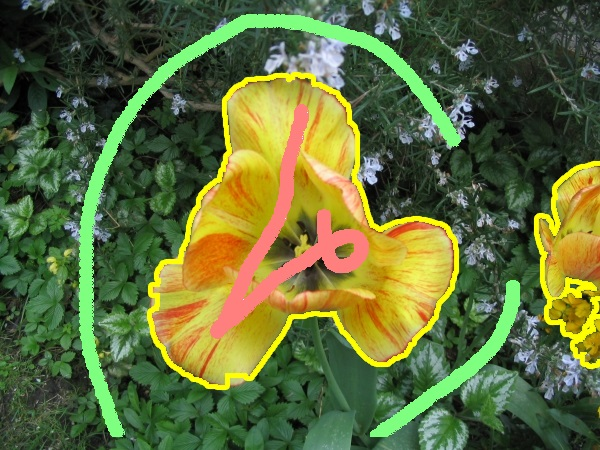
\includegraphics[width=5cm]{figures/fig7a.jpg}
    }
\subfigure[Person - $600 \times 450$]{
    \label{figure person}
    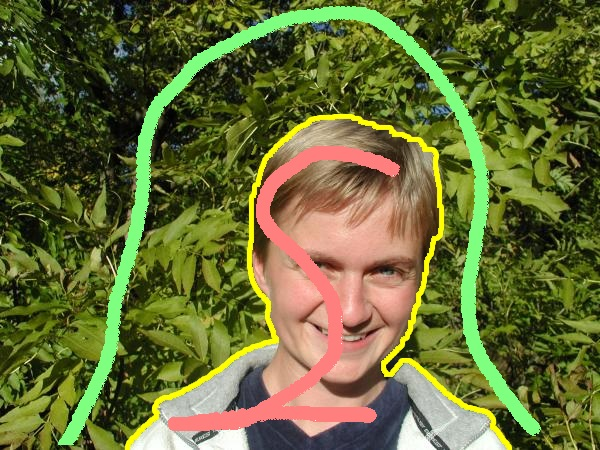
\includegraphics[width=5cm]{figures/fig7b.jpg}
    }
\subfigure[Sponge - $640 \times 480$]{
    \label{figure sponge}
    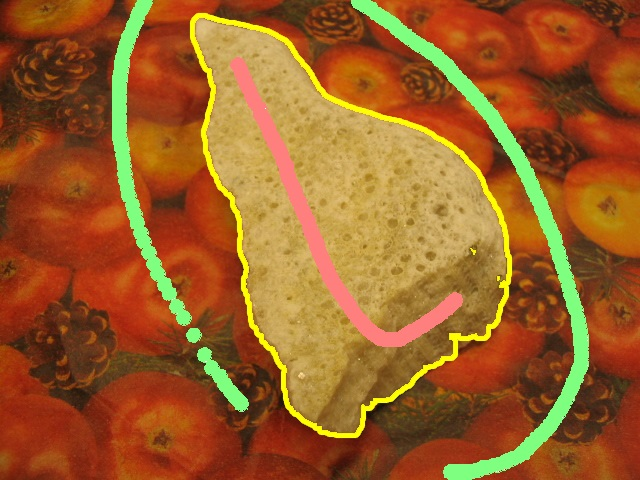
\includegraphics[width=5cm]{figures/fig7c.jpg}
    }
\\
\subfigure[Madagascar - $10800 \times 8100$]{
    \label{figure madagascar}
    \includegraphics[width=8.04cm]{figures/fig8c.jpg}
    }
\subfigure[Lower Than Atlantis - $9900 \times 7500$]{
    \label{figure lower than atlantis}
    \includegraphics[width=7.96cm]{figures/fig8d.jpg}
    }
\caption{Image Segmentation Results.
\ref{figure flower}-\ref{figure sponge}: benchmark data sets with small size.
\ref{figure lower than atlantis}-\ref{figure madagascar}: large images. \protect\footnotemark[1] \protect\footnotemark[2]
}
\label{figure image segmentation}
\end{figure*}

\paragraph*{\textbf{Video Cutout}} We use the clustering based model to build energy function.
These videos are clipped from official trailers of different films such as \textit{THE CROODS}
\footnotemark[3]\footnotetext[3]{\scriptsize TimeScapes - Trailer 2 4k 2560p: \url{http://red.cachefly.net/TimeScapes4K2560p.mp4}},
\textit{TimeScapes}
\footnotemark[4]\footnotetext[4]{\scriptsize THE CROODS - Official Trailer 3: \url{http://www.youtube.com/watch?v=xrbwgn_kRBo}} and
\textit{Life of Pi}
\footnotemark[5]\footnotetext[5]{\scriptsize Life of Pi - Trailer 2 Official: \url{http://www.youtube.com/watch?v=m7WBfntqUoA}}.
\figurename \ref{figure video cutout} shows the cutout results.

\begin{figure*}
\centering
\subfigure[TimeScapes - $2560 \times 1440 \times 30$]{
    \label{figure 4k 3d}
    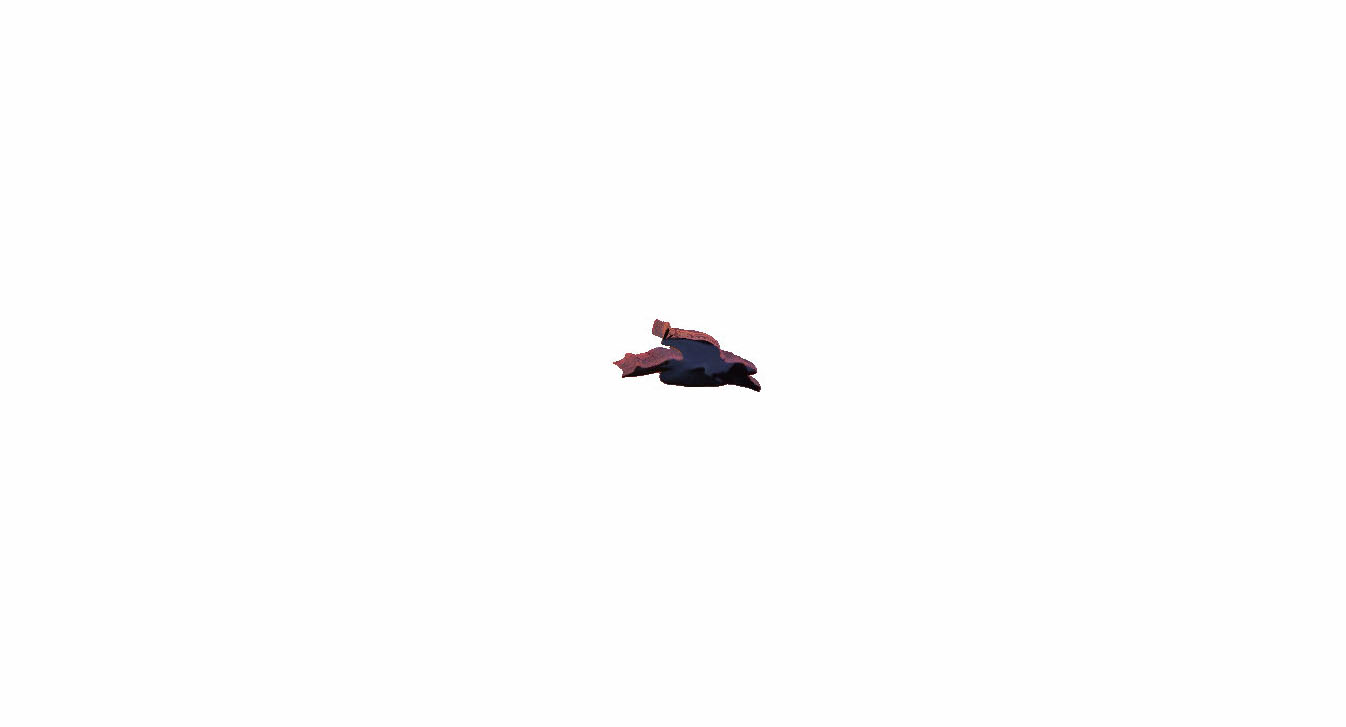
\includegraphics[width=5cm]{figures/fig16c.jpg}
    }
\subfigure[THE CROODS - $1920 \times 1080 \times 40$]{
    \label{figure eep 3d}
    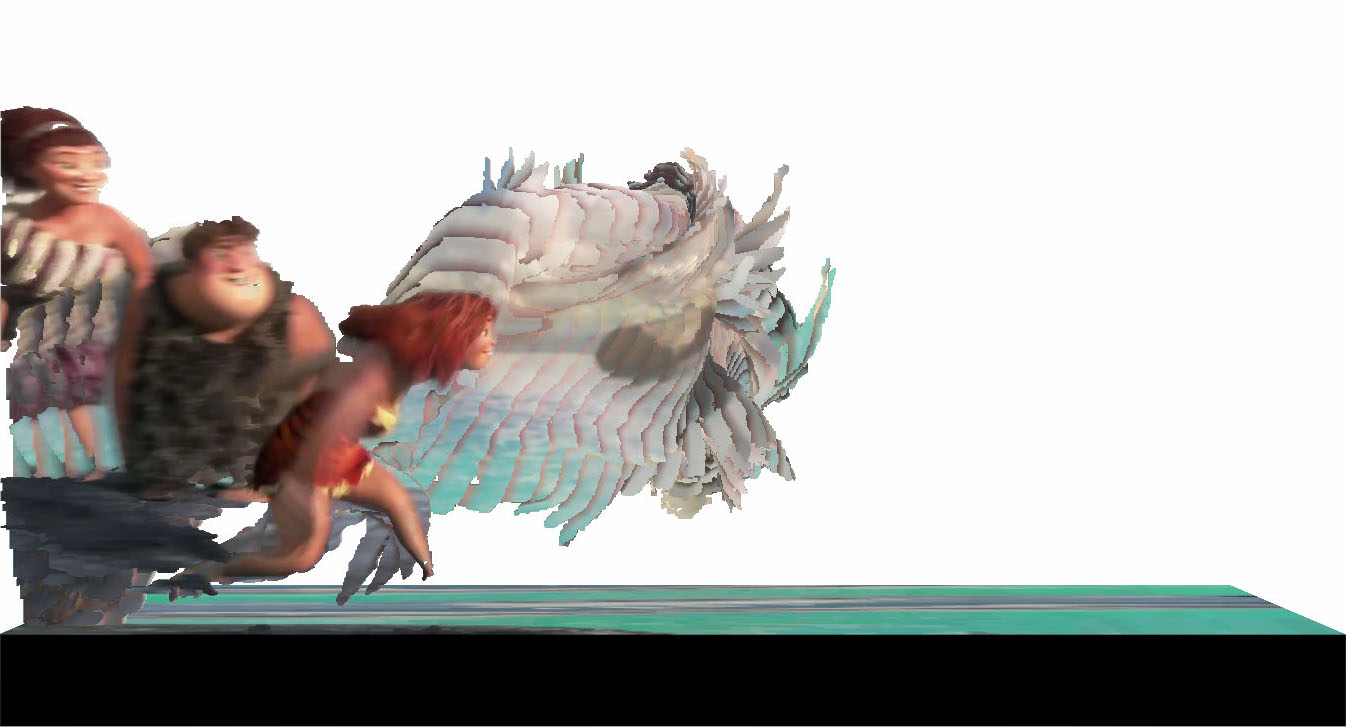
\includegraphics[width=5cm]{figures/fig14c.jpg}
    }
\subfigure[Life of PI - $1920 \times 1080 \times 36$]{
    \label{figure pi 3d}
    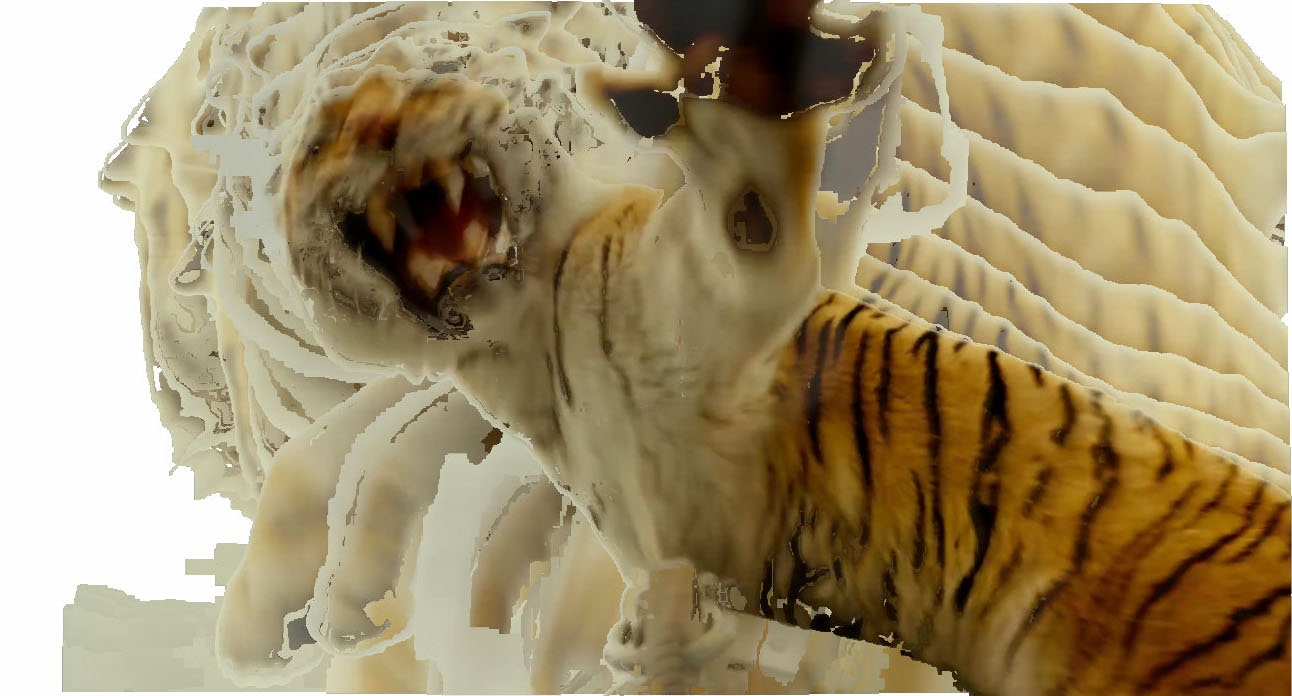
\includegraphics[width=5cm]{figures/fig15c.jpg}
    }
\\
\subfigure[TimeScapes - Frame]{
    \label{figure 4k frame}
    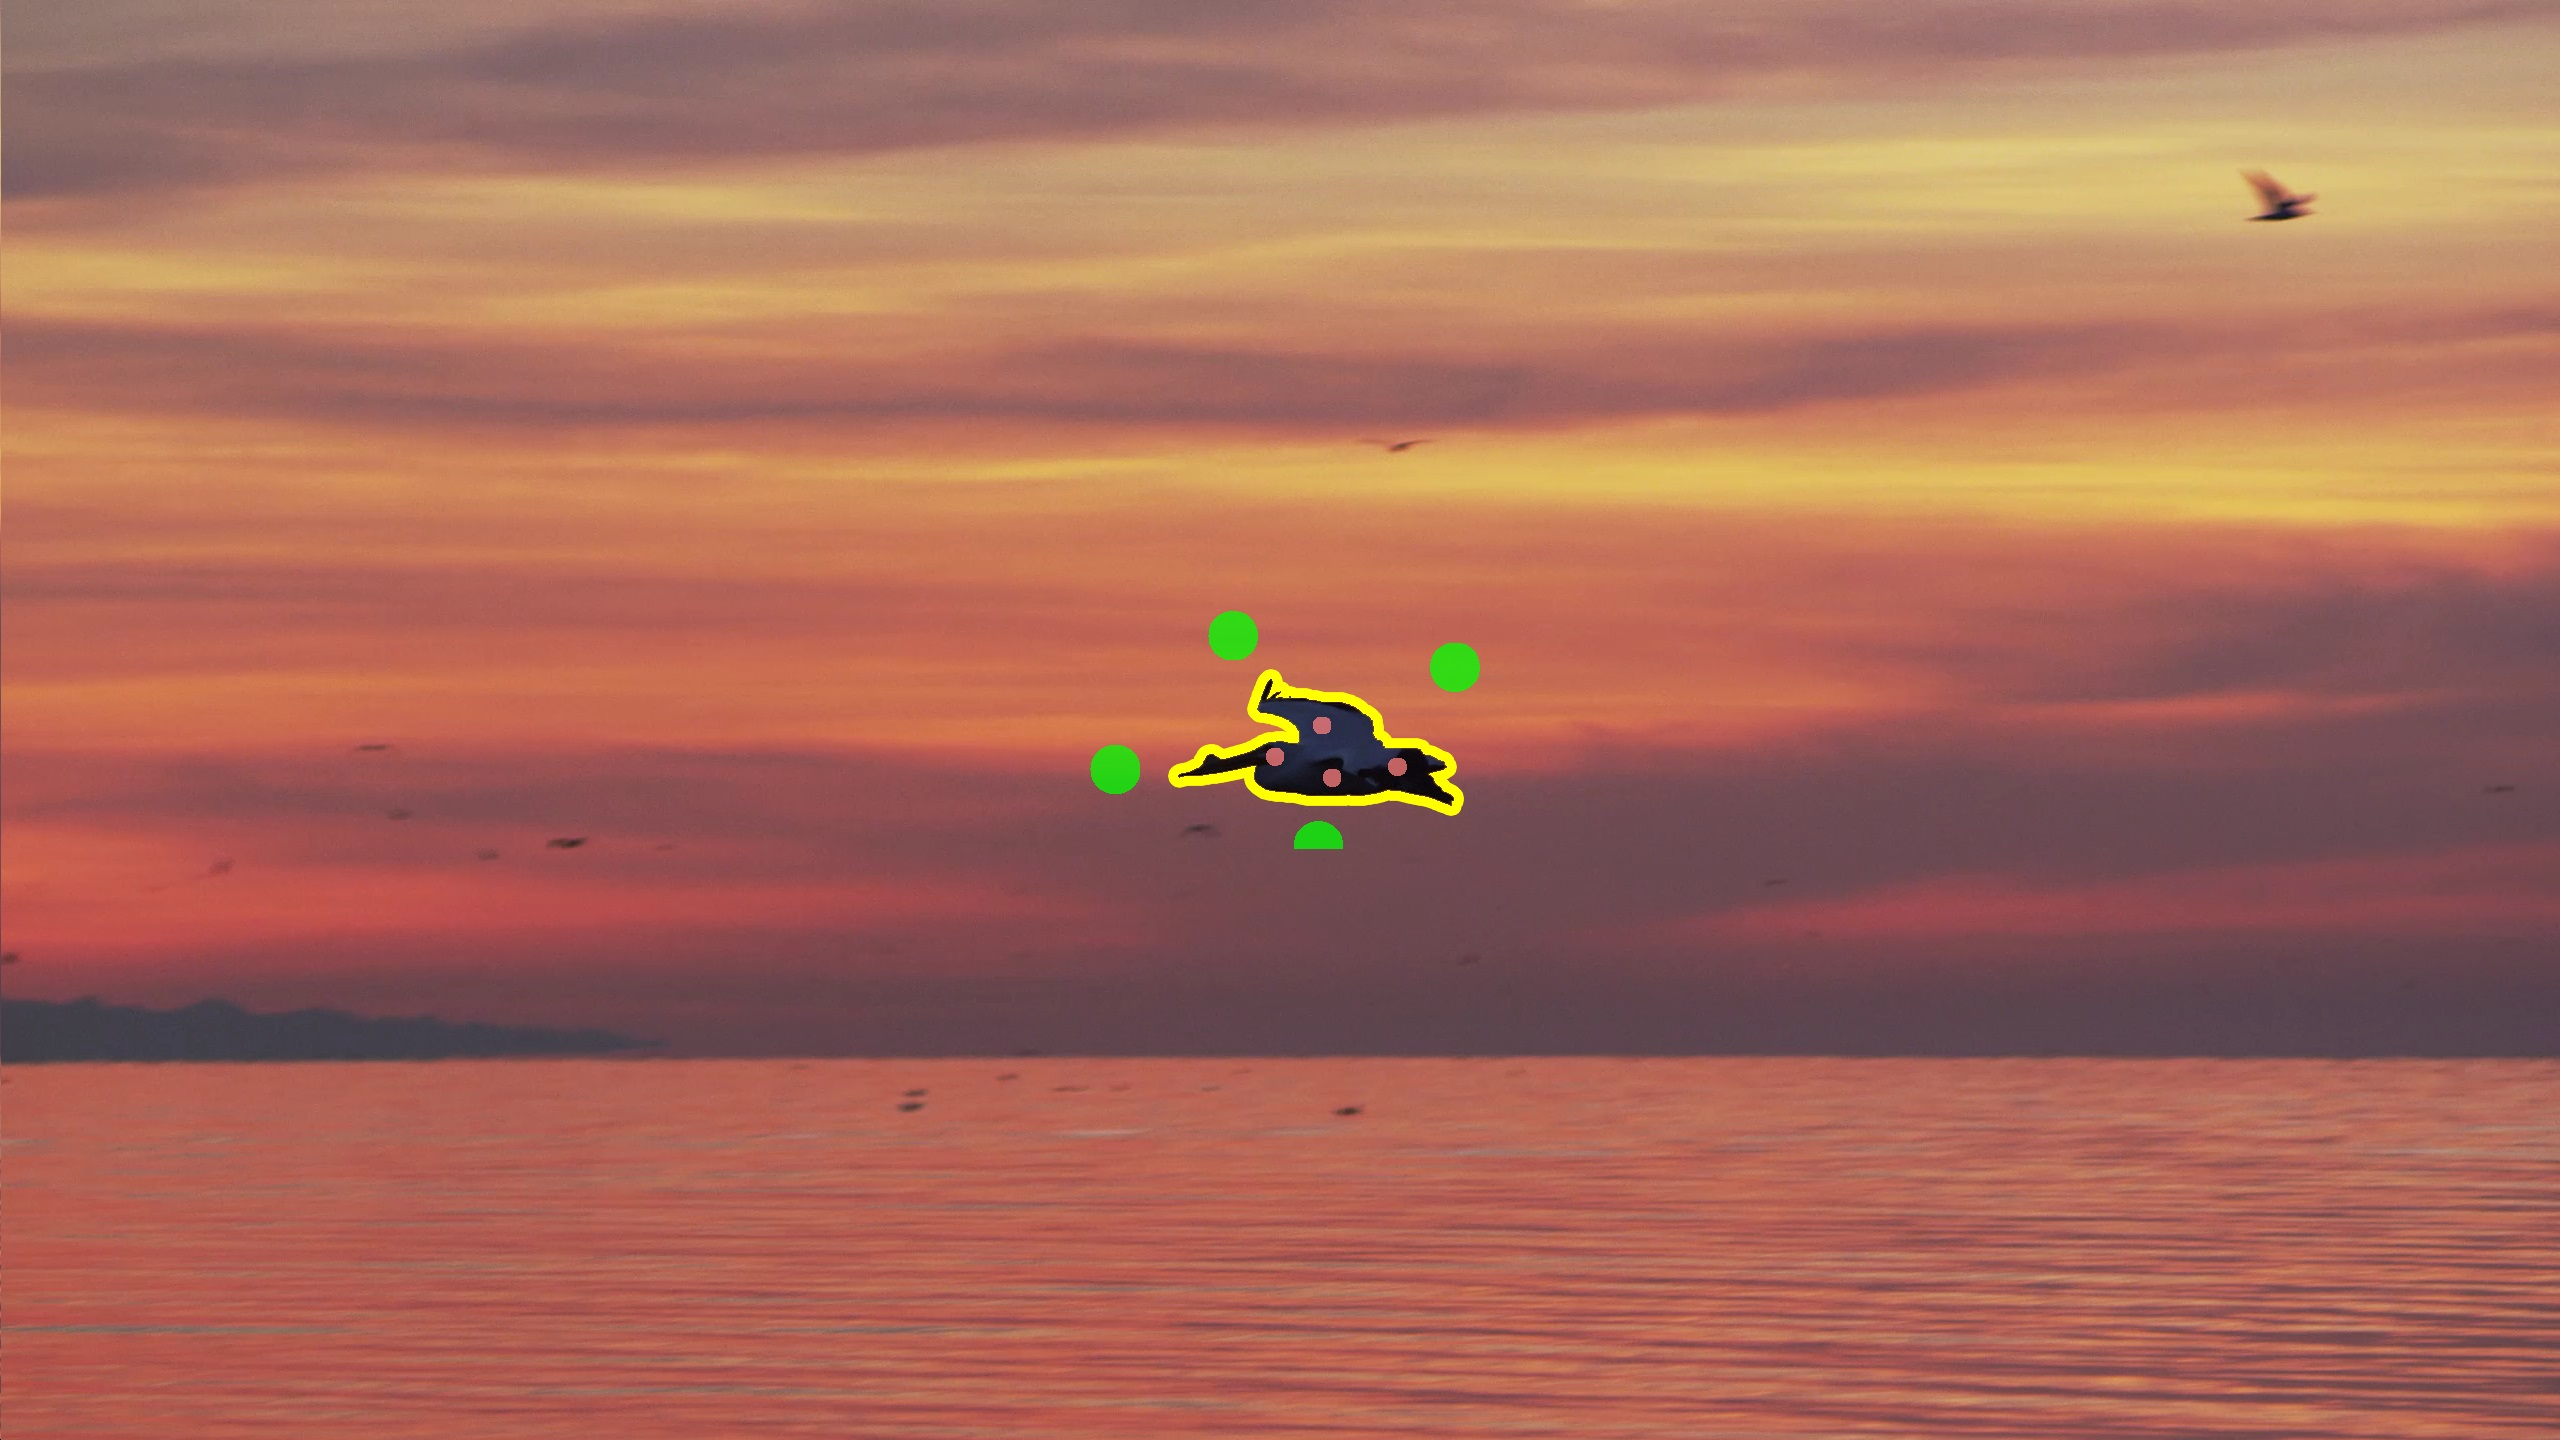
\includegraphics[width=5cm]{figures/fig16b.jpg}
    }
\subfigure[THE CROODS - Frame]{
    \label{figure eep frame}
    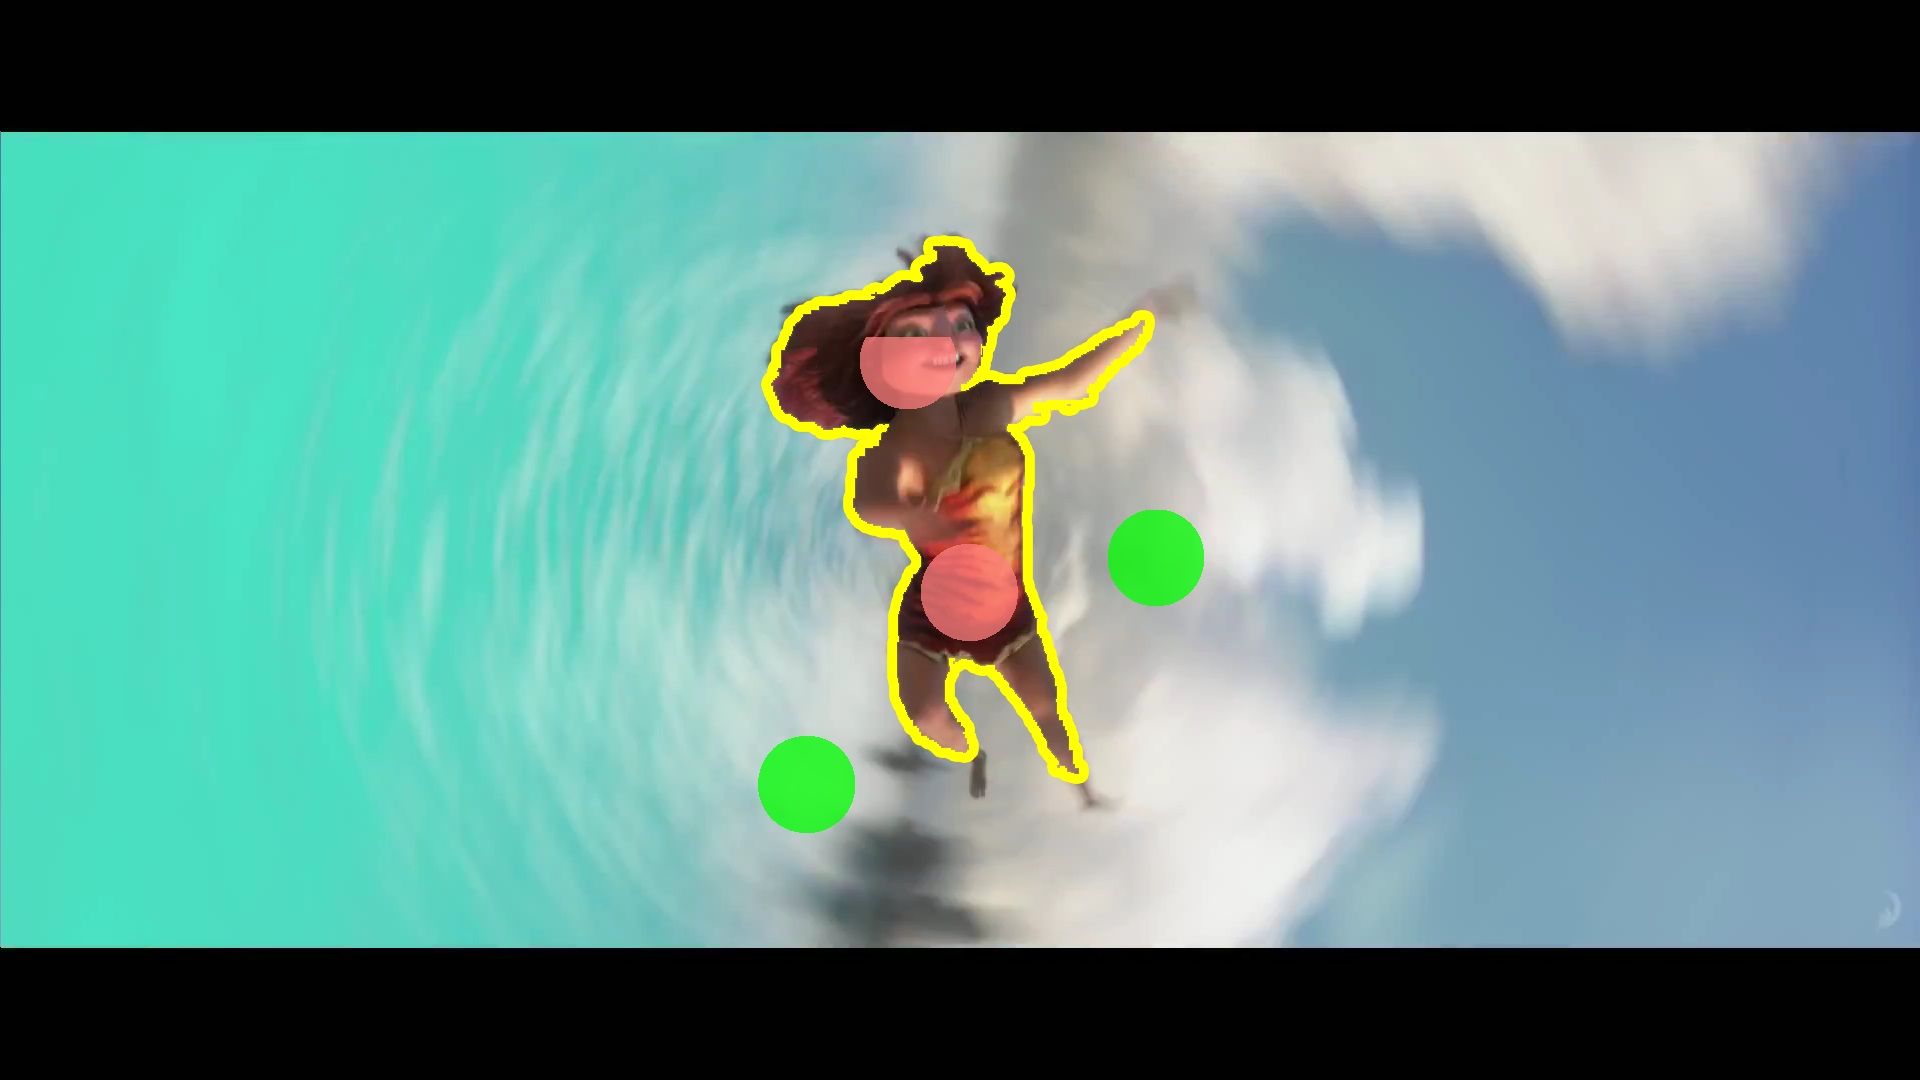
\includegraphics[width=5cm]{figures/fig14b.jpg}
    }
\subfigure[Life of PI - Frame]{
    \label{figure pi frame}
    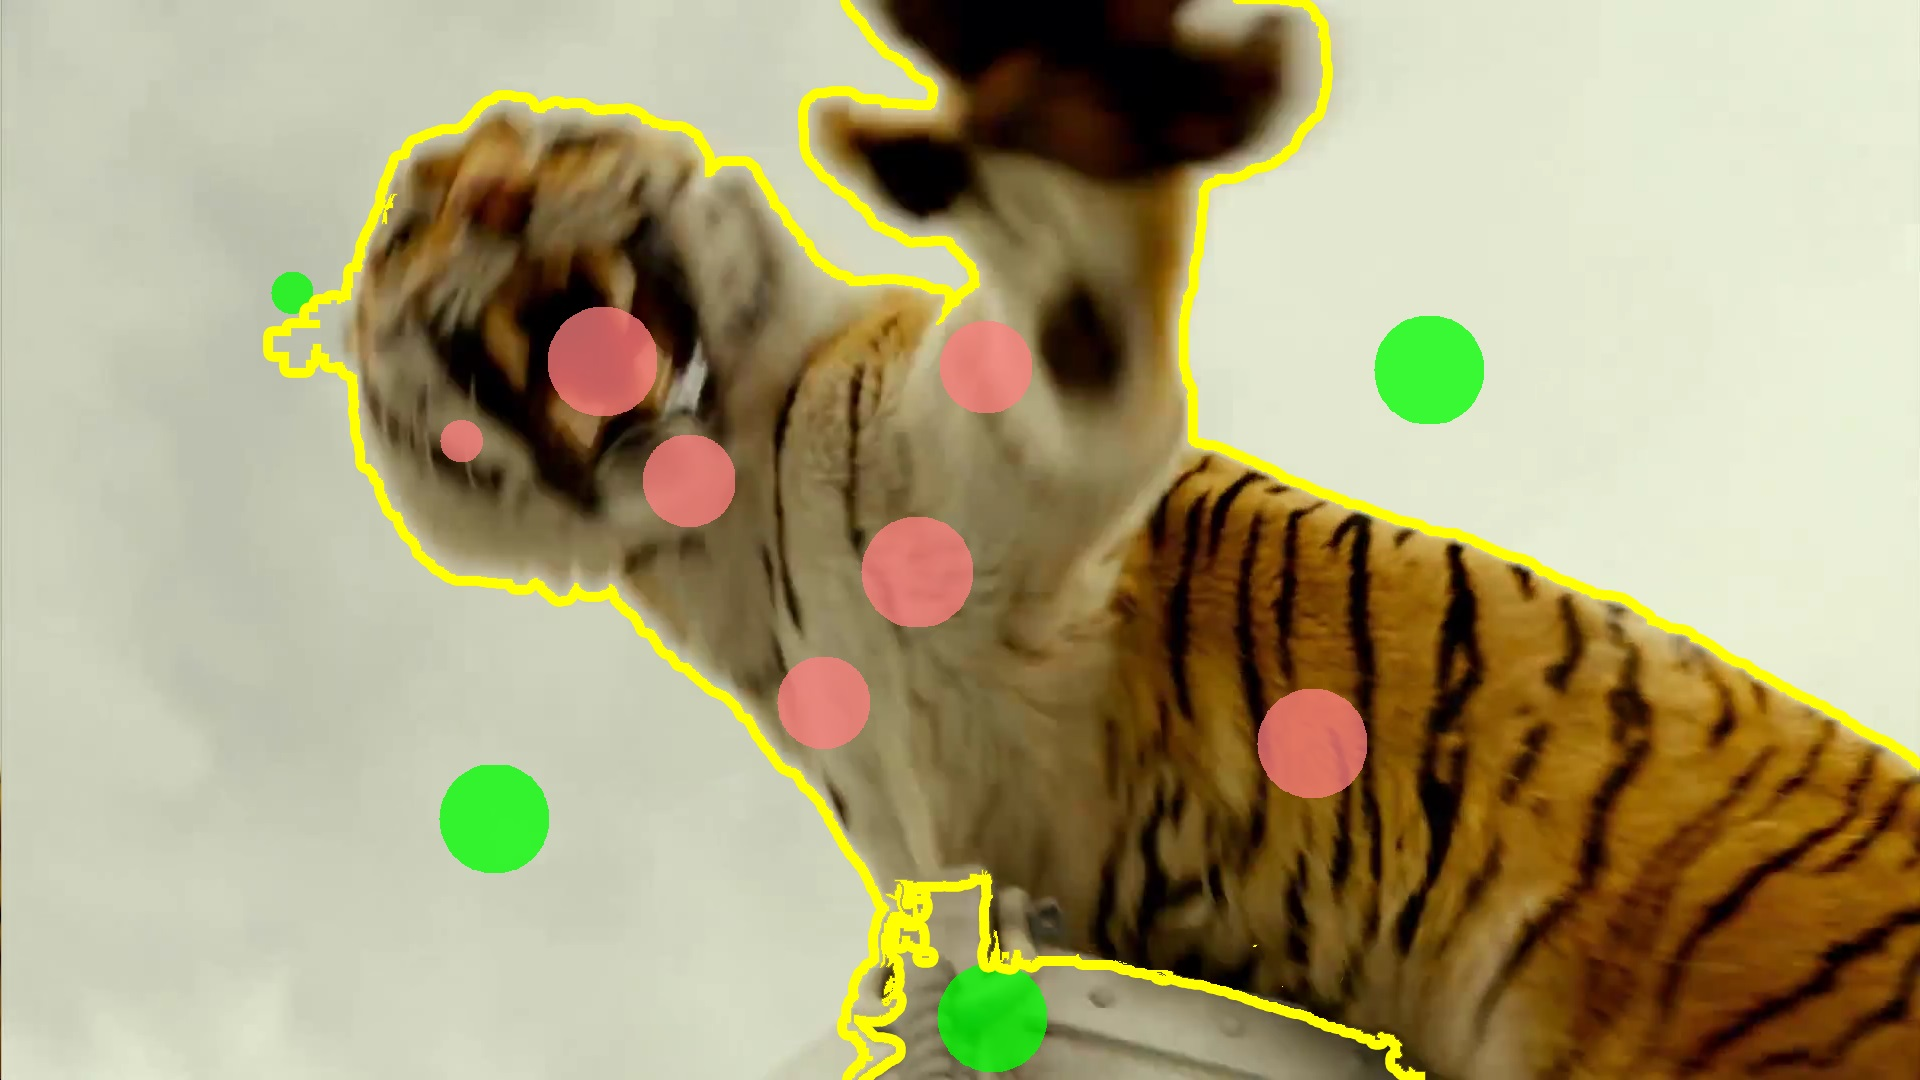
\includegraphics[width=5cm]{figures/fig15b.jpg}
    }
\caption{Video Cutout Results.
\ref{figure 4k 3d}, \ref{figure 4k frame}: the cut-out bird \protect\footnotemark[4].
\ref{figure eep 3d}, \ref{figure eep frame}: the cut-out Eep \protect\footnotemark[5].
\ref{figure pi 3d}, \ref{figure pi frame}: the cut-out tiger \protect\footnotemark[6].
}
\label{figure video cutout}
\end{figure*}

\paragraph*{\textbf{Volume Segmentation}} In terms of scalar field data sets, we use the first model to build an energy function.
Because the augmenting-paths are much longer, the computing costs are much higher compared with images.
The segmentation results of CT
\footnotemark[7]\footnotetext[7]{\scriptsize MRBrain: \url{http://www-graphics.stanford.edu/data/voldata/}} and MRI
\footnotemark[8]\footnotetext[8]{\scriptsize Lobster: \url{http://www.volvis.org/}} data sets are shown in \figurename \ref{figure volume segmentation}.

\begin{figure*}
\centering
\subfigure[MRBrain - $256 \times 256 \times 109$]{
    \label{figure mrbrain}
    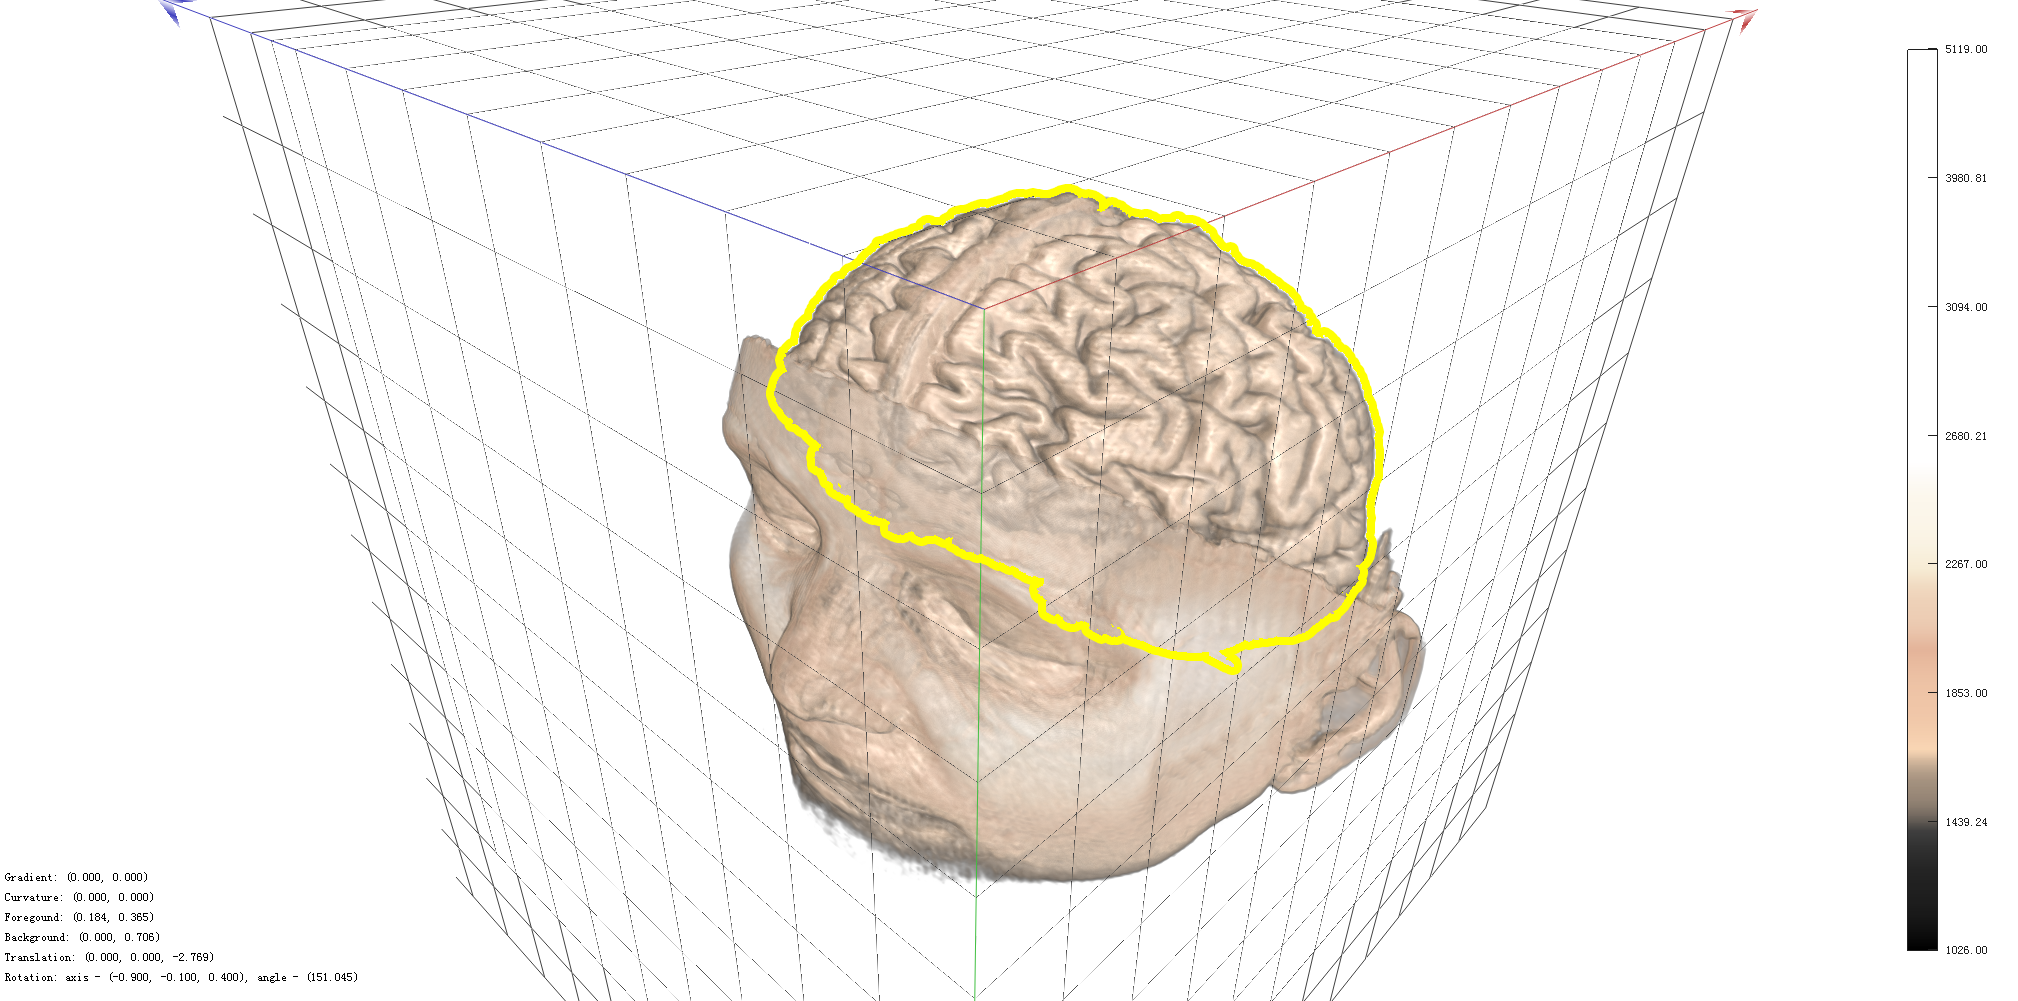
\includegraphics[width=7.5cm]{figures/fig9f.png}
    }
\subfigure[Lobster - $301 \times 324 \times 56$]{
    \label{figure lobster}
    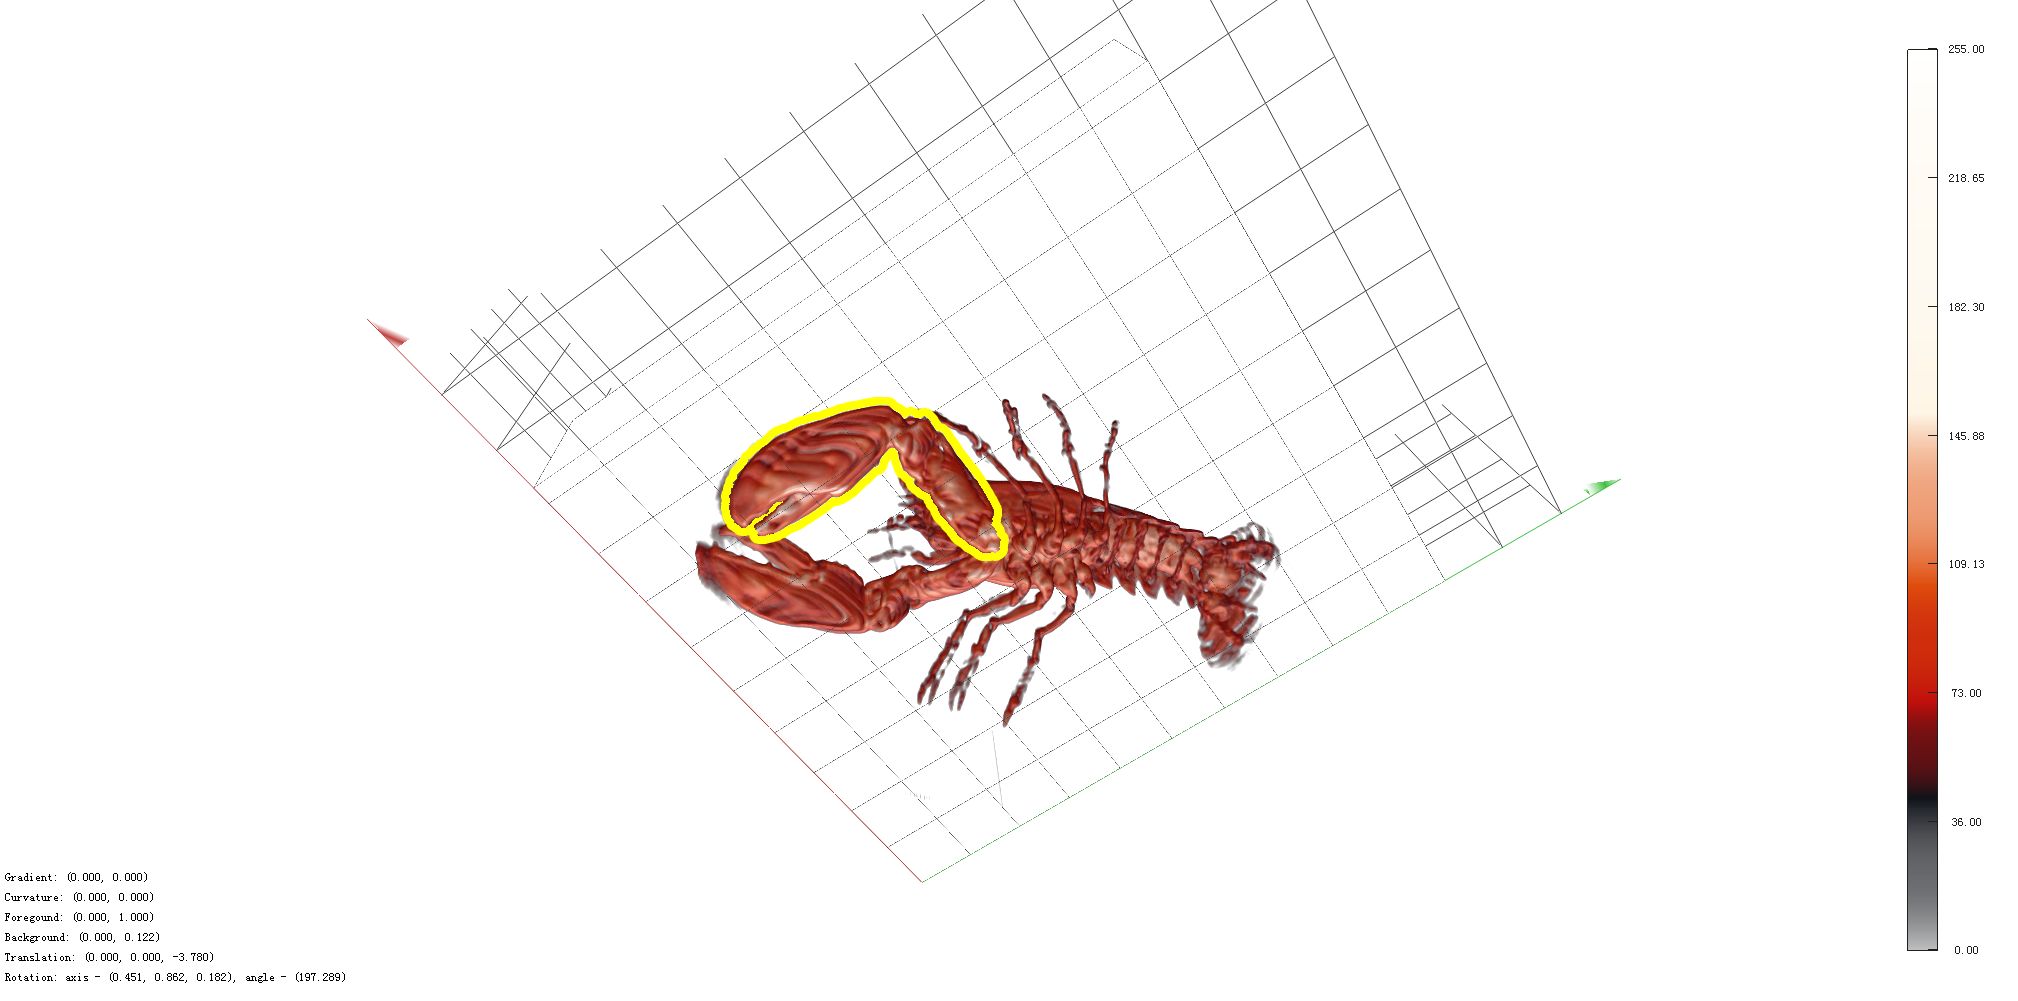
\includegraphics[width=7.5cm]{figures/fig13f.png}
    }
\caption{Volume Segmentation Results.
\ref{figure mrbrain}: MRBrain - MRI and the cutout brain \protect\footnotemark[7].
\ref{figure lobster}: Lobster - CT and the cutout claw \protect\footnotemark[8].
}
\label{figure volume segmentation}
\end{figure*}

%-------------------------------------------------------------------------
\subsection{Performance}

We first compare our method with CUDA-Cut \cite{08VN} and Fast-Cut \cite{09S, 11W} which are GPU based methods, and then with CPU based methods BK \cite{04BK} and Grid-Cut \cite{12JSH}.

\paragraph*{\textbf{GPU Based Methods}}

CUDA-Cut provides two different implementations: atomic (PushPull + Relbel) and stochastic (Push + PullRelabel).
We use the stochastic version for comparison, because it is faster.
We also observe that CUDA-Cut doesn't guarantee global convergence and it often outputs larger energies.
We divide the minimum energy by its output to measure the degree of approximation as listed in the second column of \tablename \ \ref{table gpu performance}.
Because JF-Cut and Fast-Cut always yield global optimal results, their accuracies are not listed.

We implement Fast-Cut using OpenCL and extends it to support videos (some of the optimization techniques are deprecated for generality).
To be fair, we perform global relabel once at the beginning by using the same block size and mainly compare the cost on push-relabel which is the major part of all GPU based methods
(we perform convergence detection and active block counting much less frequently).

\begin{table}
\center
\caption{GPU Based Methods}
\label{table gpu performance}
{
    \fontsize{6.5pt}{7.5pt}\selectfont
    \begin{tabular}{@{ }c|r|r|r|r|r@{ }r@{ }}
    \hline
    Instance & \multicolumn{2}{|c|}{CUDA-Cut} & Fast-Cut & JF-Cut & \multicolumn{2}{c}{Speedup} \\
    \hline
    Name        & Accuracy & Time(ms) & Time(ms) & Time(ms) & -/CUDA & -/Fast\\
    \hline
    flower      & 0.736 & 48.6  & 9.7       & 4.2       & 11.5  & 2.3\\
    4 x 4       & 0.673 & 622.2 & 262.4     & 90.0      & 6.9   & 2.9\\
    16 x 16     & -     & -     & 9636.7    & 2192.3    & -     & 4.4\\
    person      & 0.358 & 73.9  & 20.9      & 10.0      & 7.4   & 2.1\\
    4 x 4       & 0.674 & 612.0 & 290.9     & 120.7     & 5.1   & 2.4\\
    16 x 16     & -     & -     & 12131.0   & 3403.6    & -     & 3.6\\
    sponge      & 1.000 & 48.7  & 5.4       & 4.4       & 11.0  & 1.2\\
    4 x 4       & 0.973 & 637.3 & 151.7     & 31.4      & 20.3  & 4.8\\
    16 x 16     & -     & -     & 3689.5    & 595.3     & -     & 6.2\\
    \hline
    bone        & -     & -     & 5643.6    & 616.9     & -     & 9.1\\
    2 x 2 x 2   & -     & -     & 68712.3   & 6749.9    & -     & 10.2\\
    liver       & -     & -     & 6211.4    & 585.7     & -     & 10.6\\
    2 x 2 x 2   & -     & -     & 165704.3  & 16441.2   & -     & 10.1\\
    babyface    & -     & -     & 7932.5    & 830.2     & -     & 9.6\\
    2 x 2 x 2   & -     & -     & 104277.6  & 11309.2   & -     & 9.2\\
    adhead      & -     & -     & 17084.4   & 1654.6    & -     & 10.3\\
    2 x 2 x 2   & -     & -     & 115991.0  & 10511.7   & -     & 11.0\\
    \hline
    madagascar  & -     & -     & 49559.9   & 24465.4   & -     & 2.0\\
    lta         & -     & -     & 95605.9   & 51279.0   & -     & 1.9\\
    \hline
    timescapes  & -     & -     & 357.2     & 78.6      & -     & 4.5\\
    the croods  & -     & -     & 9410.7    & 1374.6    & -     & 6.8\\
    life of pi  & -     & -     & 743.4     & 80.9      & -     & 9.2\\
    \hline
    mrbrain     & -     & -     & 9381.0    & 1226.2    & -     & 7.7\\
    lobster     & -     & -     & 2892.9    & 321.5     & -     & 9.0\\
    \hline
    \end{tabular}
    \begin{tablenotes}
        \item {
        \begin{enumerate}
            \item CUDA-Cut (v1.0) - \url{http://cvit.iiit.ac.in/resources/cudacuts/}
            \item Environment - Nvidia GeForce GTX TITAN
        \end{enumerate}}
    \end{tablenotes}
}
\end{table}

\tablename \ \ref{table gpu performance} shows the performance of CUDA-Cut, Fast-Cut and our method with millisecond precision.
Because CUDA-Cut consumes too much memory, it cannot handle large date sets, even there are 6GB device memory.
For all data sets listed in \tablename \ \ref{table benchmark}, JF-Cut is faster than Fast-Cut and CUDA-Cut.
Our method achieves a maximum 20-fold speedup, see Sponge $4 \times 4$.
Larger data sets lead to higher speedups, which means our approach is more suitable for large data sets.

\begin{table}
\center
\caption{Convergence Speed}
\label{table convergence speed}
{
    \fontsize{6.5pt}{7.5pt}\selectfont
    \begin{tabular}{@{ }c|r@{ }r@{ }r|r@{ }r@{ }}
    \hline
    Instance & \multicolumn{3}{|c|}{Iterations} & \multicolumn{2}{c}{Ratios}\\
    \hline
    Name & CUDA & Fast-Cut & JF-Cut & -/CUDA & -/Fast\\
    \hline
    flower      & 155   & 41    & 10    & 15.5  & 4.1\\
    4 x 4       & 232   & 174   & 81    & 2.9   & 2.1\\
    16 x 16     & -     & 516   & 195   & -     & 2.6\\
    person      & 232   & 100   & 26    & 8.9   & 3.8\\
    4 x 4       & 232   & 203   & 88    & 2.6   & 2.3\\
    16 x 16     & -     & 692   & 366   & -     & 1.9\\
    sponge      & 155   & 31    & 14    & 11.1  & 2.2\\
    4 x 4       & 232   & 114   & 27    & 8.6   & 4.2\\
    16 x 16     & -     & 234   & 84    & -     & 2.8\\
    \hline
    bone        & -     & 265   & 125   & -     & 2.1\\
    2 x 2 x 2   & -     & 410   & 184   & -     & 2.2\\
    liver       & -     & 498   & 170   & -     & 2.9\\
    2 x 2 x 2   & -     & 1721  & 697   & -     & 2.5\\
    babyface    & -     & 512   & 194   & -     & 2.6\\
    2 x 2 x 2   & -     & 876   & 413   & -     & 2.1\\
    adhead      & -     & 518   & 197   & -     & 2.6\\
    2 x 2 x 2   & -     & 439   & 175   & -     & 2.5\\
    \hline
    madagascar  & -     & 1344  & 609   & -     & 2.2\\
    lta         & -     & 1344  & 668   & -     & 2.0\\
    \hline
    timescapes  & -     & 36    & 13    & -     & 2.8\\
    the croods  & -     & 68    & 34    & -     & 2.0\\
    life of pi  & -     & 32    & 10    & -     & 3.2\\
    \hline
    mrbrain     & -     & 516   & 282   & -     & 1.8\\
    lobster     & -     & 214   & 104   & -     & 2.1\\
    \hline
    \end{tabular}
}
\end{table}

The convergence speed of different methods is shown in \tablename \ \ref{table convergence speed}.
Because the augmenting paths in volume data sets are longer than in images, volume data sets need more iterations.
Our method has higher convergence speeds which are more than twice the rates of Fast-Cut and almost 10-fold to CUDA-Cut.

\paragraph*{\textbf{CPU Based Methods}}

We download the latest version of BK (V3.03) and Grid-Cut (V1.1) and compile them to get the 64-bit programs.
The reason why we choose 64-bit programs is that for large data sets, such as adhead $2 \times 2 \times 2$ and TimeScapes, BK requires a contiguous memory which is larger than 4GB.
We use the same compiler settings for comparison, see the table notes in \tablename \ \ref{table cpu performance}.

\begin{table}
\caption{CPU Based Methods}
\label{table cpu performance}
{
    \fontsize{6.5pt}{7.5pt}\selectfont
    \begin{tabular}{@{ }c|r|r@{ }r|r@{ }r@{ }r@{ }r@{ }}
    \hline
    Instance & BK & \multicolumn{2}{c}{Grid-Cut} & \multicolumn{4}{c}{JF-Cut}\\
    \hline
    Name        & Total     & 1 Thread & 8 Threads & Total & -/BK  & -/GC-1 & -/GC-8\\
    \hline
    flower      & 29        & 18     & 6       & 6     & 4.7   & 2.9    & 1.0\\
    4 x 4       & 495       & 131    & 89      & 101   & 4.9   & 1.3    & 0.9\\
    16 x 16     & 9850      & 2392   & 1462    & 1575  & 6.3   & 1.5    & 0.9\\
    person      & 29        & 9      & 7       & 14    & 2.1   & 0.6    & 0.5\\
    4 x 4       & 494       & 121    & 92      & 118   & 4.2   & 1.0    & 0.8\\
    16 x 16     & 9111      & 2069   & 1377    & 2417  & 3.8   & 0.9    & 0.6\\
    sponge      & 28        & 7      & 6       & 13    & 2.2   & 0.6    & 0.5\\
    4 x 4       & 466       & 93     & 79      & 41    & 11.5  & 2.3    & 1.9\\
    16 x 16     & 7537      & 1531   & 1265    & 595   & 12.7  & 2.6    & 2.1\\
    \hline
    bone        & 5761      & 867    & 519     & 421   & 13.7  & 2.1    & 1.2\\
    2 x 2 x 2   & 204874    & 32057  & 20402   & 4707  & 43.5  & 6.8    & 4.3\\
    liver       & 10769     & 3254   & 3916    & 305   & 35.3  & 10.7   & 12.8\\
    2 x 2 x 2   & 855279    & 237593 & 256249  & 7923  & 107.9 & 30.0   & 32.3\\
    babyface    & 8940      & 2619   & 1501    & 459   & 19.5  & 5.7    & 3.3\\
    2 x 2 x 2   & 809026    & 231592 & 233656  & 5825  & 138.9 & 39.8   & 40.1\\
    adhead      & 23192     & 6517   & 4149    & 980   & 23.7  & 6.6    & 4.2\\
    2 x 2 x 2   & 223934    & 41414  & 21274   & 7921  & 28.3  & 5.2    & 2.7\\
    \hline
    madagascar  & 114673    & 29658  & 12269   & 13730 & 8.4   & 2.2    & 0.9\\
    lta         & 104006    & 32055  & 13139   & 24275 & 4.3   & 1.3    & 0.5\\
    \hline
    timescapes  & 18175     & 3640   & 2741    & -     & -     & -      & -\\
    the croods  & 12603     & 2883   & 2115    & 906   & 13.9  & 3.2    & 2.3\\
    life of pi  & 11700     & 3925   & 2162    & 209   & 55.9  & 18.8   & 10.3\\
    \hline
    mrbrain     & 3902      & 599    & 597     & 798   & 4.9   & 0.8    & 0.7\\
    lobster     & 7028      & 1428   & 657     & 229   & 30.7  & 6.2    & 2.9\\
    \hline
    \end{tabular}
    \begin{tablenotes}
        \item {
        \begin{enumerate}
            \item BK (v3.03) - \url{http://pub.ist.ac.at/~vnk/software.html}
            \item Grid-Cut (v1.1) - \url{http://gridcut.com/downloads.php}
            \item Compiler Settings for GCC (v4.9.0) -O3 -march=native -mtune=generic -DNDEBUG
            \item Environment - Intel (R) Core i7-3770 and AMD Radeon HD 7990
        \end{enumerate}}
    \end{tablenotes}
}
\end{table}

\tablename \ \ref{table cpu performance} compares the performance of BK, Grid-Cut and our method.
Our method's speedup over Gird-Cut increases with the data scale, except for some data sets.
Compared with Grid-Cut, we achieve a maximum 3-fold speedup (sponge $16 \times 16$) for images, a 20-fold speed up (life of pi) for videos and a 40-fold speedup (babyface $2 \times 2 \times 2$) for volume data sets.
With its parallel version (8 threads), the maximum speedups are 2-fold for images, 10-fold for videos and 40-fold for volume data sets.

We also observe that there exists a notable variant.
The decisive factor may be the graph topology.
The reason is that in volume data sets most of the terminal-edges have zero capacities, while in images most of them are positive, which will greatly affect the convergence speed.
These speedups are lower than of GPU based methods, because there exist big differences between CPU based methods (based on augmenting-path) and GPU based methods (based on push-relabel).
In summary, for large data sets our method significantly outperforms other methods.
